\documentclass[titlepage,dvipdfmx,uplatex,a4j,12pt]{beamer}
\usepackage{listings}
\usepackage{media9}
\usepackage{graphicx}
\usepackage{hyperref}
\usepackage{amssymb}
\usepackage{amsthm}
\usepackage{booktabs}
\usepackage{amsmath}
\lstset{%
    basicstyle={\ttfamily\small},
    commentstyle={\ttfamily\small},
    frame=tb,
    breaklines=true,
    lineskip=-0.5ex,
    tabsize=2,
    numbers=left,
    numberstyle={\ttfamily\scriptsize},
    columns=[l]{fullflexible},
}
\renewcommand\lstlistingname{ソースコード}
\renewcommand\proofname{\bf 証明}

\title{OS自作入門第一}
\author{toku\_san}
\AtBeginSection[]{
    \begin{frame}
        \vfill
        \centering
        \begin{beamercolorbox}[sep=8pt,center,shadow=true,rounded=true]{title}
            \usebeamerfont{title}\insertsectionhead\par%
        \end{beamercolorbox}
        \vfill
    \end{frame}
}
\begin{document}

\maketitle

\begin{frame}{内容}
    \tableofcontents
\end{frame}

\section{始めに}

\begin{frame}[fragile]{自己紹介}
    \begin{figure}[ht]
        \centering
        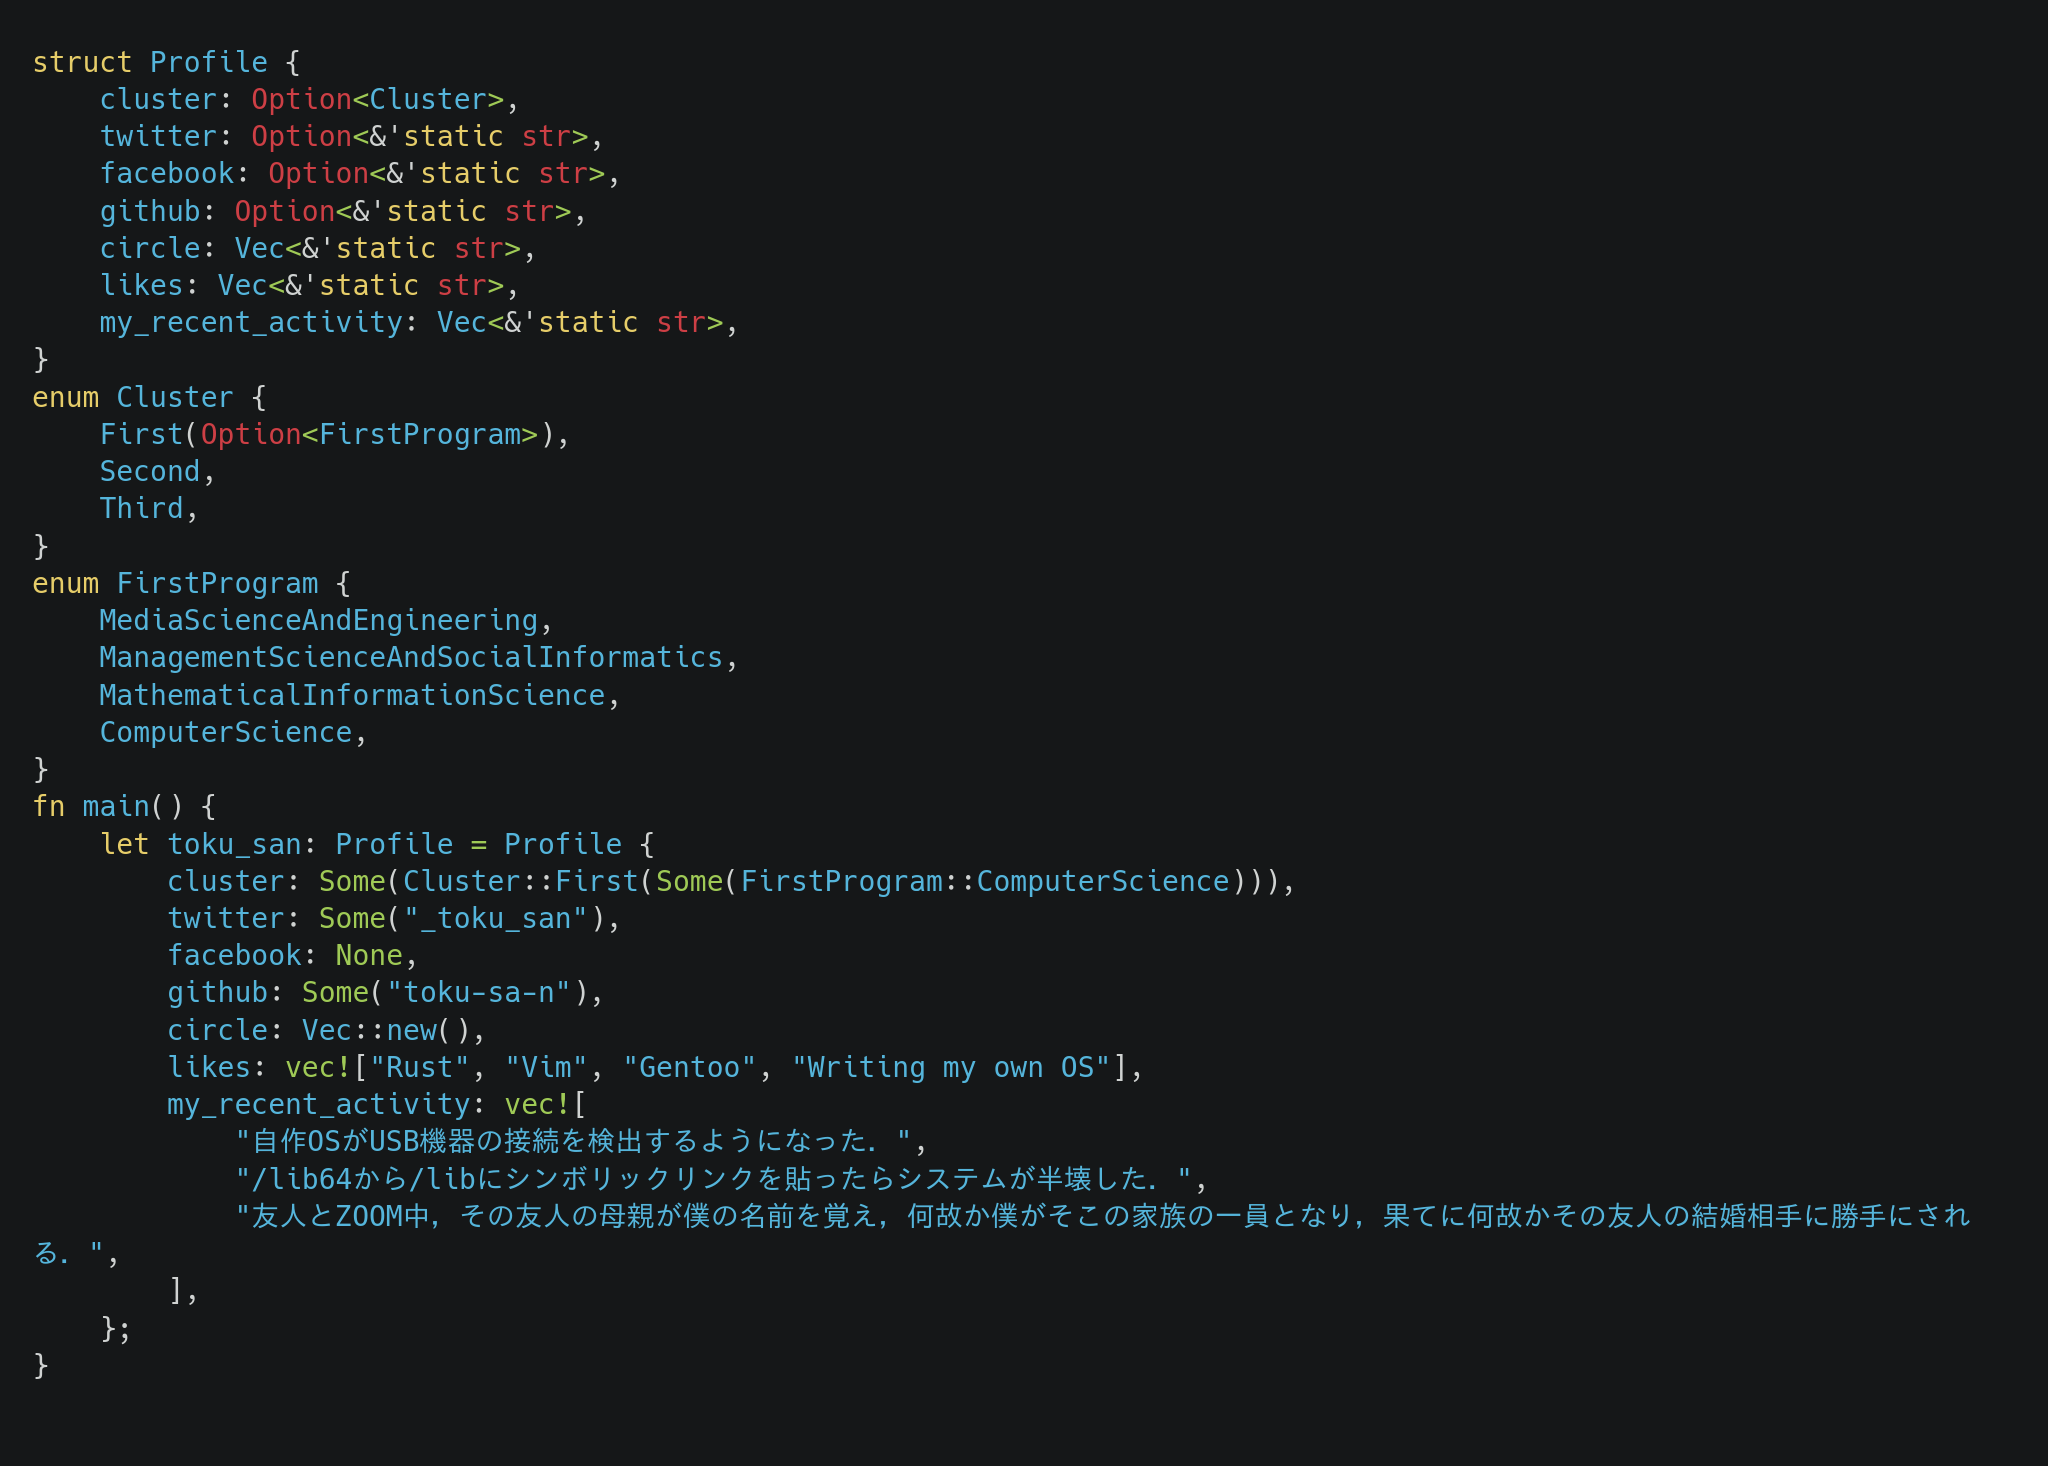
\includegraphics[width=\linewidth]{carbon.png}
        \label{fig:carbon.png}
    \end{figure}
\end{frame}

\begin{frame}{このスライドの在り処}
    https://github.com/toku-sa-n/uec\_18\_os\_slide
\end{frame}

\section{OS開発とは}

\begin{frame}{デモンストレーション}
    \href{run:demo.mp4}{動画}
\end{frame}

\begin{frame}{OSがやっているようなこと}
    \begin{itemize}
        \item デバイスの操作
        \item 画面描画
        \item プロセス操作
        \item システムコールの提供
    \end{itemize}
    など
\end{frame}

\begin{frame}{デバイスの操作}
    割り込み処理を用いる.

    \begin{itemize}
        \item マウスを動かした時
        \item キーボードのキーを押した時
    \end{itemize}

    OSは割り込みが起きた時にデータを読み出す.
\end{frame}

\begin{frame}{マウスを動かすと入手出来る情報}
    \begin{table}[h]
        \tiny
        \caption{パケットの中身}
        \centering
        \begin{tabular}{llllllll}
            \toprule
            Y overflow & X overflow & Y sign bit & X sign bit & Always 1 & Middle Btn & Right Btn & Left Btn \\
            \multicolumn{8}{c}{X movement}  \\
            \multicolumn{8}{c}{Y movement}
            \\ \bottomrule
        \end{tabular}
    \end{table}
    出典:https://wiki.osdev.org/Mouse\_Input
\end{frame}

\begin{frame}{割り込み記述子表}
    \begin{table}[h]
        \caption{Interrupt Descriptor Table (=IDT)}
        \centering
        \begin{tabular}{lcl}
            \toprule
            番号 & $\cdots$ & ポインタ\\ \midrule
            $\vdots$ & $\vdots$ & $\vdots$ \\
            0xd & $\cdots$ & 0x334334334  \\
            $\vdots$ & $\vdots$ & $\vdots$ \\
            0x40 & $\cdots$ & 0x334334334334    \\
            $\vdots$ & $\vdots$ & $\vdots$ \\   \bottomrule
        \end{tabular}
    \end{table}
\end{frame}

\begin{frame}{例外}
    IDTには例外に関する記述も行なう.
    \begin{itemize}
        \item 一般保護例外 (General Protection Fault = GPF)
        \item ベージフォルト
        \item ゼロ除算
    \end{itemize}
    など.
\end{frame}

\begin{frame}{画面描画}
    Video RAM (VRAM) と呼ばれるメモリを弄る.

    メモリの大きさ:width * height * bpp\footnote{bits per pixel} / bits\_per\_bytes
\end{frame}

\begin{frame}[fragile]{画面描画の実例}
    ディスプレイの解像度が1920$\times$1080の時に,座標(33,4)を赤(\#FF0000)にする.(座標は0-based)

    \begin{lstlisting}[language={}, label=code:vram, caption=コード]
        let vram = Vram{base: 0x334_334_334, x_len: 1920, y_len: 1080};
        let ptr = vram.base + 4 * vram.x_len + 33;

        *(ptr as *mut u8) = 0;
        *((ptr + 1) as *mut u8) = 0;
        *((ptr + 2) as *mut u8) = 0xff;
    \end{lstlisting}
    (base: VRAMの開始アドレス)
\end{frame}

\begin{frame}{OS作成に必要なもの}
    \begin{itemize}
        \item アセンブリ言語の知識(ほぼ必須)
        \item $\mathrm{\left( C\left( ++ \right)?|D|Rust|Go|Ada \right)}$などの知識(オプション)
        \item 英語(オプション)
    \end{itemize}
\end{frame}

\begin{frame}[fragile]{アセンブリ言語の知識(ほぼ必須)}
    一部の処理はC等で書くことが出来ない.

    \begin{lstlisting}[language=, label=, caption=割り込み記述子表の設定]
        lidt [0x334334334]
    \end{lstlisting}

    \begin{lstlisting}[language={}, label=, caption=上記のコードをRustのインラインアセンブリで書いた例]
        asm!("lidt [0x334334334]");
    \end{lstlisting}
\end{frame}

\begin{frame}{特定のプログラミング言語の知識}
    \begin{itemize}
        \item RubyやPythonなどでOSを書くのは恐らく無理.
            \begin{itemize}
                \item その処理系がOSに依存しているため.
            \end{itemize}
        \item その他の言語であっても,OSに依存する機能は使えない.
            \begin{itemize}
                \item \lstinline{printf}など.
                \item OSに依存しないものは使用可能(最大値計算など).
            \end{itemize}
        \item アセンブリ言語だけでOSを書くことも可能.
    \end{itemize}
\end{frame}

\begin{frame}{英語}
    \begin{itemize}
        \item 読解能力
            \begin{itemize}
                \item アーキテクチャの規格書などは英語で書かれている.
            \end{itemize}
        \item 記述能力
            \begin{itemize}
                \item 使用しているライブラリに対するプルリクエスト.
                \item フォーラムへの質問の投稿.
            \end{itemize}
    \end{itemize}
\end{frame}

\section{参考文献など}

\begin{frame}{参考文献}
    \begin{itemize}
        \item 30日でできる!OS自作入門
            \begin{itemize}
                \item 30日でできる(できるとは言っていない).
                \item GUIを備えたOSを作ることができる. 楽しい.
                \item 内容が古い部分がある(フロッピー,PS/2マウスやキーボード,32ビットアーキテクチャ).
            \end{itemize}
    \end{itemize}
\end{frame}

\begin{frame}{参考文献}
    \begin{itemize}
        \item Writing an OS in Rust
            \begin{itemize}
                \item https://os.phil-opp.com/
                \item RustでのOSの書き方が載っている.
            \end{itemize}
    \end{itemize}
\end{frame}

\begin{frame}{参考文献}
    \begin{itemize}
        \item OSDev.org
            \begin{itemize}
                \item https://wiki.osdev.org/
                \item OSを制作する際に必要な様々な情報が載っている.
                \item フォーラム:https://forum.osdev.org/もおすすめ
            \end{itemize}
    \end{itemize}
\end{frame}

\begin{frame}{参考文献}
    \begin{itemize}
        \item Intel® 64 and IA-32 Architectures Software Developer Manuals
            \begin{itemize}
                \item https://software.intel.com/

                    content/www/us/en/develop/articles/intel-sdm.html
                \item x86\_64やx86に関する各種規格が載っている.
                \item 基本的にこの規格に沿っていくことになる.
            \end{itemize}
    \end{itemize}
\end{frame}

\begin{frame}{参考文献}
    \begin{itemize}
        \item オペレーティングシステム 設計と実装 第3版
            \begin{itemize}
                \item MINIX3の開発者が,MINIX3を題材としてOSの解説をしている.
            \end{itemize}
    \end{itemize}
\end{frame}

\begin{frame}{ライブラリ等}
    \begin{itemize}
        \item rust-osdevが公開しているライブラリ群
            \begin{itemize}
                \item https://github.com/rust-osdev
                \item rust-osdevはRustでOSを書くコミュニティ
                \item このコミュニティが公開しているx86\_64クレートやuefi-rsクレートは非常に便利
            \end{itemize}
    \end{itemize}
\end{frame}

\begin{frame}{自作OSの紹介}
    \begin{itemize}
        \item Ramen OS
            \begin{itemize}
                \item https://github.com/toku-sa-n/ramen
                \item 現在製作中のOS.
                \item Rustで記述.現在はUSB接続のキーボードを動かすことを目標としている.
            \end{itemize}
    \end{itemize}
\end{frame}

\end{document}
